\section{Genetic Operators}\label{sec:genetic_operators}
As per the EvoHyp toolkit \cite{pillay2017evohyp}, the genetic operators used included reproduction, crossover and mutation. Detailed by Koza and Poli \cite{koza2005genetic}, reproduction entails copying the selected individual program to the new population as is; crossover entails randomly selecting a crossover point in each of 2 parents and swapping the subtrees rooted at these points; and, mutation entails randomly selecting a point in an individual and replacing the subtree rooted at that point with a randomly created subtree.

Furthermore, every operator is associated with a probability which determines the likelihood that it will be used to select the next individual for the new population. The probability for crossover was selected as 0.8, the probability for mutation was selected as 0.1 and the probability for reproduction was also selected as 0.1. In addition, a maximum tree depth of 20 was applied as a constraint to offspring; and, the maximum mutation depth for subtrees created by the mutation operator was 4. With the selection methods and genetic operators having been identified, figure \ref{fig:breeding_pipeline} depicts the entire breeding pipeline for generating a new population from an existing population.

\begin{figure}[H]
\centering
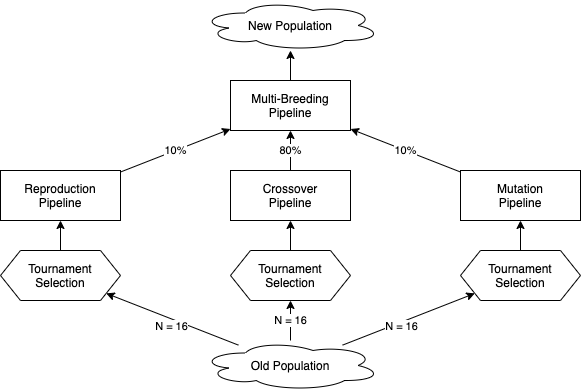
\includegraphics[width=\textwidth]{report/05_genetic_operators/breeding_pipeline.png}
\caption{Breeding Pipeline}
\label{fig:breeding_pipeline}
\end{figure}